\chapter{Introduction\label{intro}}

The act of \textit{searching} has become so deeply ingrained in the modern society that we tend to take it for granted, not only assuming it normal to have immediate and easily accessible information on the tip of our thumbs, but expecting it: a study from 2004 showed that users were not willing to wait more than ten seconds for a page to load \citep{waitTime}. Fast forward twenty years and nowadays even a couple seconds holdup would be unacceptable, thus query retrieval needs to be fast. Blazingly fast in fact, since we need to account for all the delays typical of a gargantuan structure as big as the modern web, and, as the reader probably knows, it is \textit{not} a good idea to rely on memory's performances increasing over time: the smart way to tackle this problem is via research and development of efficient algorithms, and exactly which type should be self-evident from the title of this document. The problem of the set intersection constitutes the backbone of every query resolver in a (web) search engine, since every word in a query is interpreted as a collection of documents' IDs which contains it. \\
In this survey-style paper we will first explain what searching (i.e., querying) entails, show how a document (e.g., a web page) can be transformed into word tokens which are then further processed into inverted indexes, and, finally, we will see a collection of algorithms that concern themselves with intersecting sets, meaning finding common elements between two or more comparable collections. 

\section{How Do We Search?}

\begin{figure}[ht] 
\begin{center}
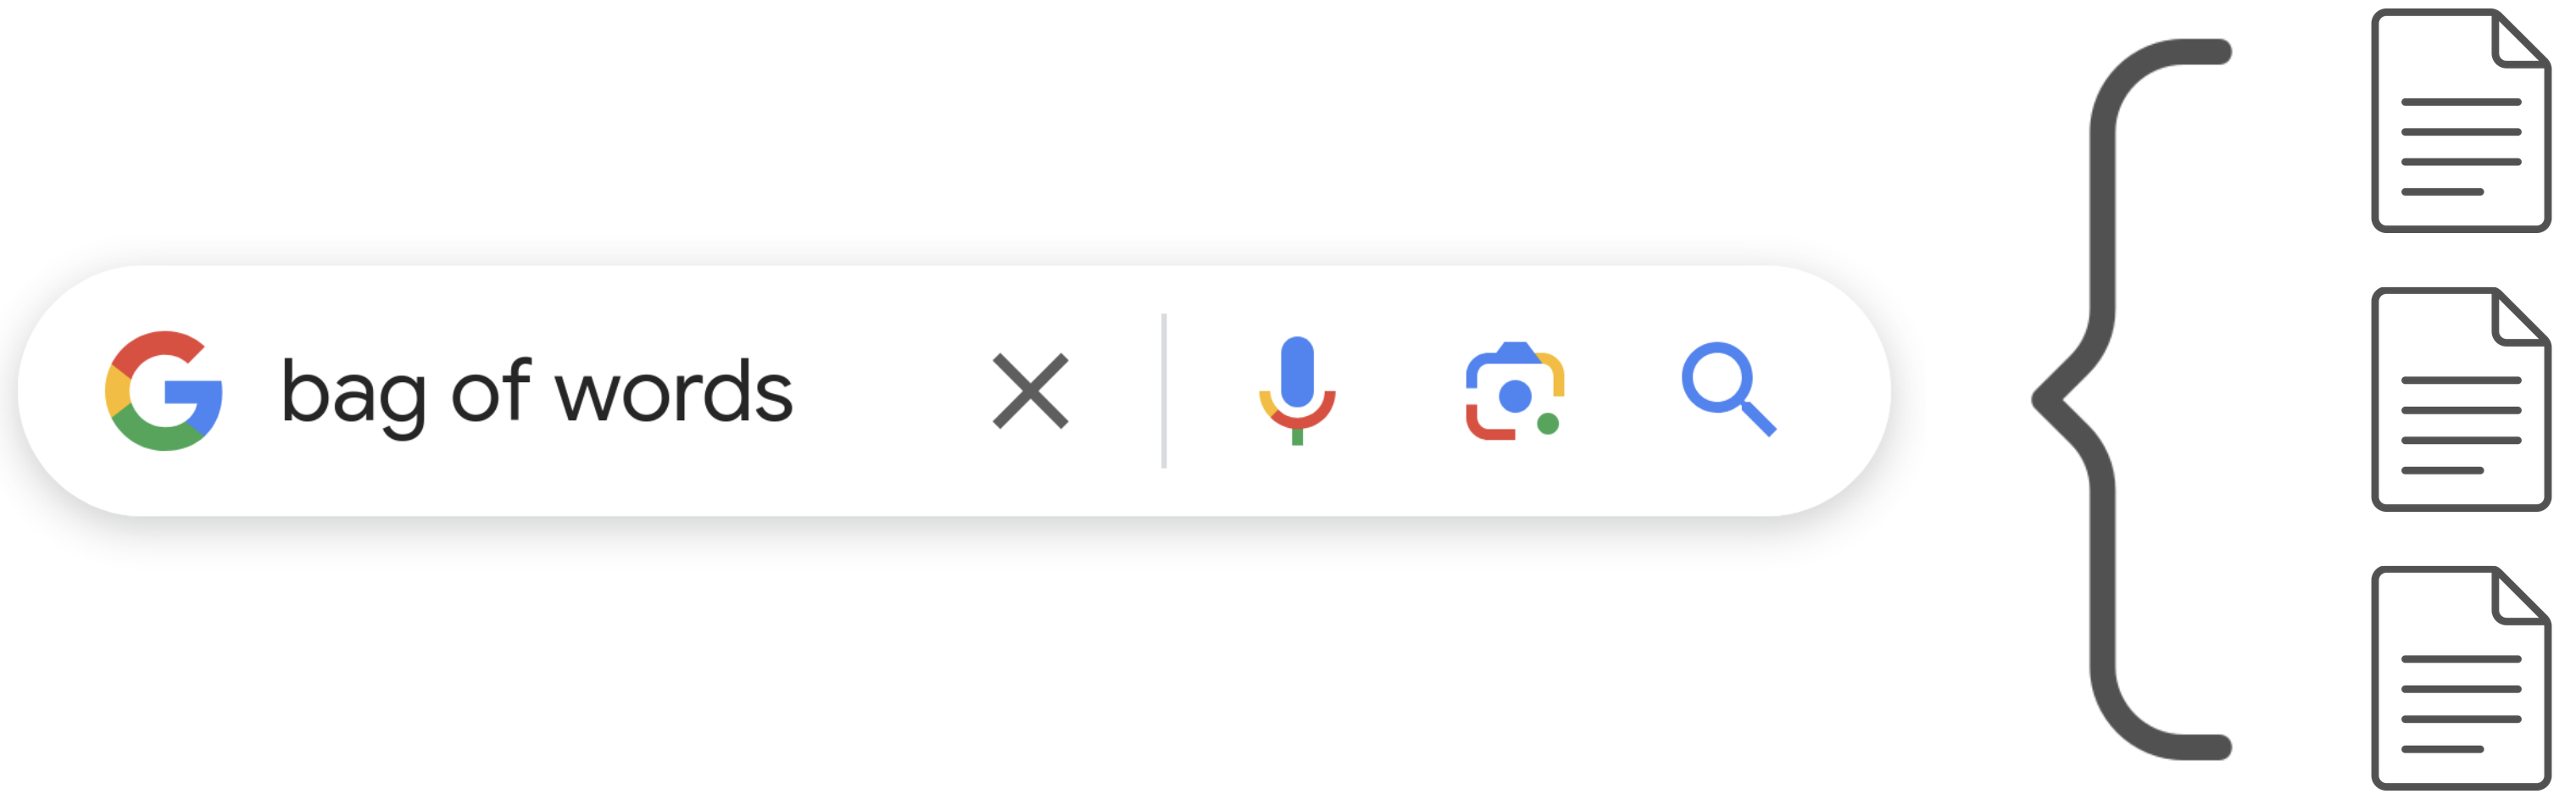
\includegraphics[width=.8\textwidth]{imgs/query_bagofwords.png}
\caption{From a bag of words to a set of documents\label{fig:bagtodocs}}
\end{center}
\end{figure}


Generally speaking, a query is called a \textit{bag of words}, and finding its result means computing which documents contain all word tokens that are being searched for [\ref{fig:bagtodocs}]. Let's make and example: word \verb+abiura+ is contained in documents number \verb+[31, 42, 127]+, while word \verb+bitonto+ is contained in documents number \verb+[20, 42, 72]+. \\
Thus \verb|query = (abiura,bitonto)| will return the result \verb+42+. \\

\begin{figure}[ht] 
\begin{center}
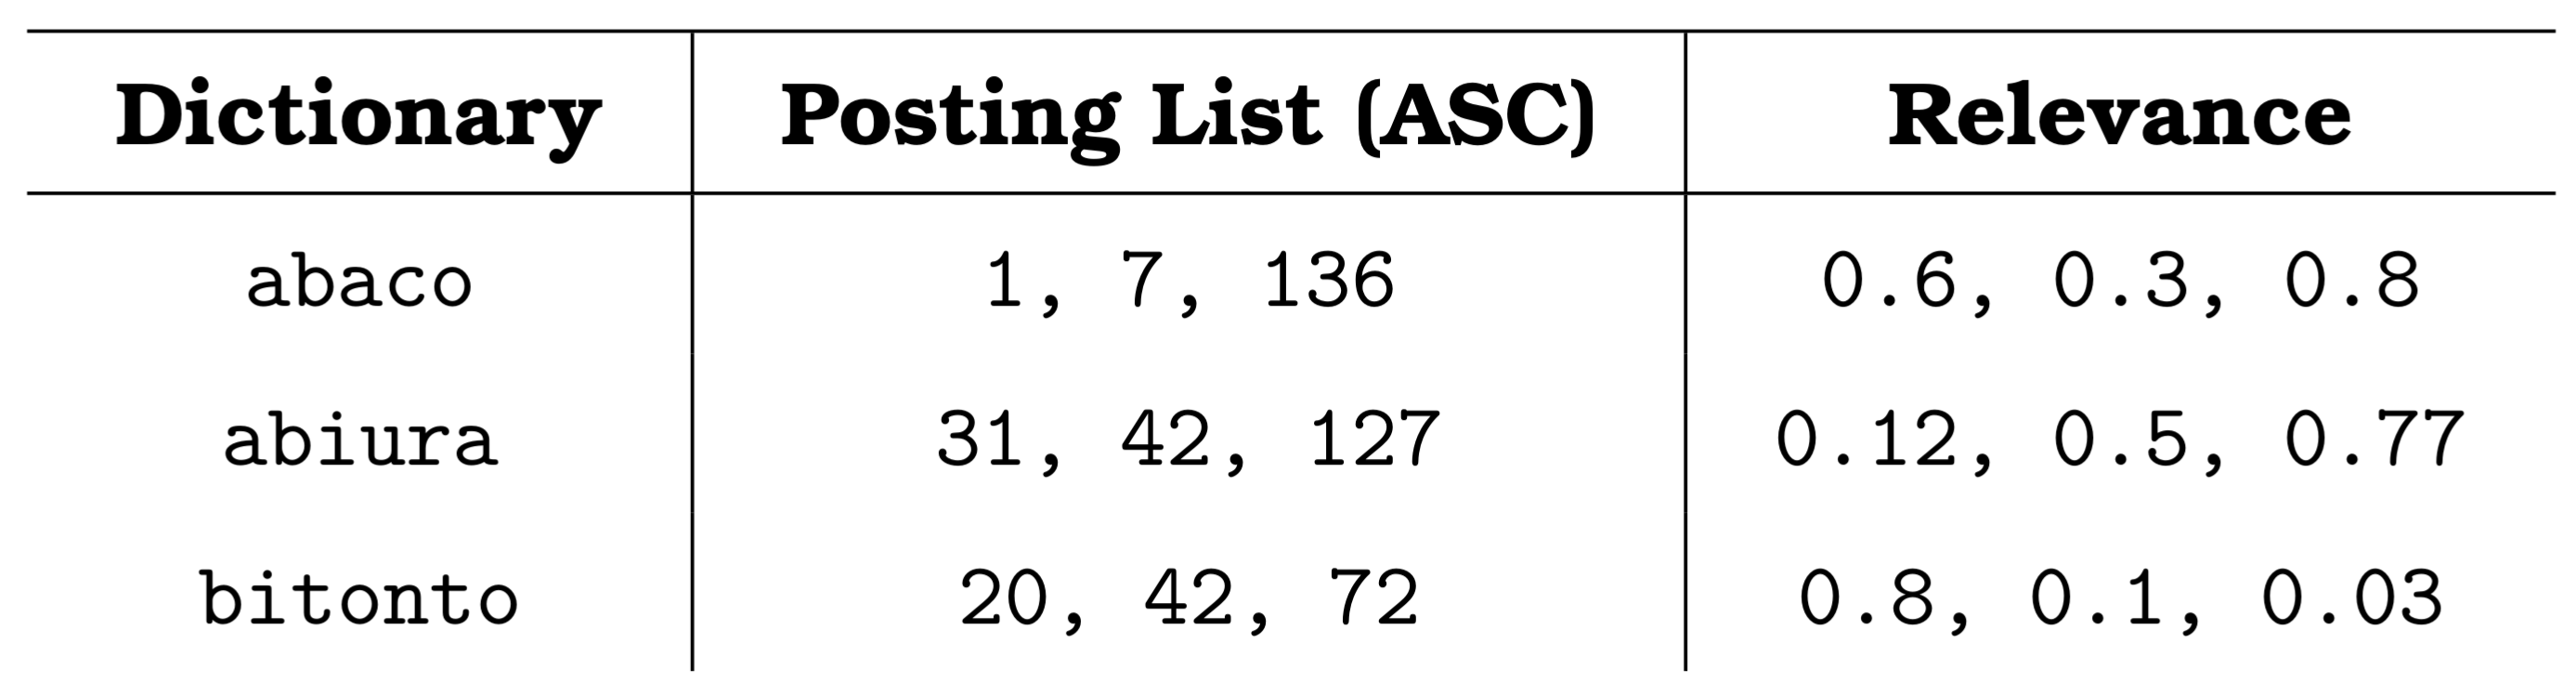
\includegraphics[width=.8\textwidth]{imgs/table_of_words.png}
\caption{Table of word tokens\label{fig:table_wtokens}}
\end{center}
\end{figure}

Both The example above [\ref{fig:table_wtokens}] and all the algorithms we will see in this survey consider the problem of searching as the problem of complete intersection, but modern search engine (e.g., Google)  leverage input relevance and filter unneeded outputs to obtain faster and better results. Unfortunately finding information about how they do it is near impossible, since everything is covered by trade secret. \\
Let's now see what inverted indexes are and how we can obtain them starting from a document corpus.

